\chapter{Motivación y antecedentes}
\label{ch:antecedentes}

\noindent Año tras año, en todos los países occidentales, el modelo de negocio de las plataformas de alquiler vacacional con apartamentos turísticos no deja de crecer \cite{juanjocerezo2018}. La forma en la que se organizan las vacaciones, los viajes de negocios y cualquier actividad que incluya pernoctar, está adaptándose a una nueva forma de economía colaborativa. La repercusión que esto tiene en el mercado es positiva, haciendo que nuestro país vea aumentada su capacidad para acoger turistas, de forma que el producto interior bruto recibe un fuerte impulso.\\
No obstante, este modelo de economía colaborativa no está al acceso de todo el mundo, ya que la atención de los clientes es algo que requiere una importante inversión de tiempo, que no siente resulta compatible con la vida laboral o personal de los potenciales anfitriones.\\
Algunos de los problemas que requieren de la atención y el tiempo de los propietarios de viviendas de uso turístico, han sido automatizados por empresas que, a cambio de tarifas mensuales o anuales, ofrecen diferentes servicios a los clientes:
\begin{itemize}
\item Evitar un exceso de huéspedes para una misma habitación. La mayoría de los propietarios de viviendas de uso turístico, tienen sus anuncios en varias plataformas, como Airbnb, Booking, Homeaway, etc. Esto puede provocar que diferentes personas alquilen la misma propiedad en idénticas fechas, produciendo así un fenómeno de sobre venta, lo cual resulta castigado en la mayoría de los casos por medio de sanciones en dichas plataformas. Para solucionar este problema, las estas plataformas ofrecen ya soluciones\footnote{\url{https://www.airbnb.es/help/article/99/como-sincronizo-mi-calendario-de-airbnb-con-otro-calendario}}, pero además existen múltiples empresas que permiten sincronizar los calendarios, haciendo que al recibir una reserva en una plataforma, las demás queden deshabilitadas para tales fechas, acabando así con este indeseado fenómeno.
\item Responder a los clientes. La mayoría de plataformas de alquiler vacacional, incluyen en su software la posibilidad de ofrecer respuestas automáticas\footnote{\url{https://partner.booking.com/es/ayuda/reservas/}}, de manera que los propietarios de las viviendas no se vean obligados a responder uno por uno a los clientes.
\item Apertura de puertas de forma automática. Existen además empresas que se dedican a implantar sistemas automáticos para la apertura de puertas\footnote{\url{https://raixer.com/funcionamiento/abrir-puertas-automaticamente/}}. Estas aperturas se realizan a través de una petición de usuario, bien por medio de una llamada telefónica, o bien por medio de una aplicación que se puede descargar en Android e iOS.
\item Cálculo automatizado de precios. Optimizar los precios de una vivienda turística puede resultar un auténtico quebradero de cabeza para aquellos que quieran hacerlo de forma acertada. Las grandes cadenas hoteleras funcionan por medio de algoritmos automatizados que actualizan constantemente los precios en función de muchas variables, como la demanda, el tiempo restante, etc. En la actualidad, existen también plataformas que permiten actualizar dichos precios de forma automatizada\footnote{\url{https://hello.pricelabs.co/}}, de manera que el propietario, a cambio de un pago mensual, pueda ahorrarse una cantidad considerable de tiempo y potenciar al máximo la optimización de sus precios.

\end{itemize}

\noindent Como puede observarse, las empresas tecnológicas han apostado por el mercado de los alojamientos turísticos para emprender negocios, optimizando cada vez más esta forma de comercio. Sin embargo, los anfitriones siguen contando con una importante carga de trabajo, que repercute en su capacidad de incorporarse a este modelo de economía colaborativa.

Las motivaciones principales de este trabajo de fin de grado pasan por mejorar, de manera bidireccional, la experiencia de los huéspedes y los anfitriones, así como acercar a estos últimos la posibilidad de poder incluir este modelo de negocio pasivo en su economía personal. A continuación se mencionarán algunas de estas motivaciones de manera más detallada.

\section{Automatización completa del proceso de reserva} 
\label{sec:automatizacion-completa-del-proceso-de-reserva}

\noindent La posibilidad de incluir un sistema automatizado por completo, o uno semi automatizado, puede ser decisiva a la hora de que una persona se decida por el modelo de negocio de las viviendas de uso turístico.

El trabajo y los asuntos personales suelen requerir de una cantidad importante de recursos para las personas, que no siempre disponen del tiempo y la energía suficiente para atender a los turistas, y debido a ello, deciden abandonar este tipo de inversiones.

Este aspecto podría ser distinto, sin embargo, si por medio de un sistema automatizado, el anfitrión pudiera tener la tranquilidad de saber que su negocio se está gestionando solo, ya que de esta manera si podría plantearse esta inversión sabiendo que no le requerirá invertir tiempo de forma diaria. Un sistema que atienda de principio a fin al cliente, organizando cada reserva y ofreciendo el acceso a la vivienda, podría dar una solución definitiva a este problema y, de esta manera, abrir este terreno a multitud de potenciales anfitriones.

\section{Uso de aplicaciones de mensajería instantánea} 
\label{sec:uso-de-aplicaciones-de-mensajeria-instantanea}

\noindent En la actualidad, recientes estudios \cite{itreseller2019} afirman que el 85 por ciento de los españoles utiliza aplicaciones de mensajería instantánea. Para cualquier modelo de negocio, incluir una nueva tecnología en la que la curva de aprendizaje sea mínima, tendrá siempre un impacto positivo en la supervivencia de su fase inicial. En este caso, hacer que todo este sistema se automatice por medio de aplicaciones de mensajería instantánea hará que se facilite su uso a la inmensa mayoría de la población.

Además, según un estudio \cite{samuelfernandez2019} realizado por Telefónica, se ha demostrado que el 95,1\% de los españoles prefiere enviar un mensaje a realizar una llamada, por lo que se demuestra, una vez más, la validez de este método como forma de gestión de estos negocios al alza.

\section{Estado del arte}

\noindent El internet de las cosas, según Wikipedia\footnote{\url{https://es.wikipedia.org/wiki/Internet_de_las_cosas}} se define como la interconexión digital de objetos cotidianos por internet.

Su principal objetivo es el de facilitar la vida de las personas, evitando tener que hacer una importante cantidad de trabajos manuales, y en muchas ocasiones, optimizando los resultados obtenidos respecto a un humano.

\subsection{Historia del internet de las cosas}

\noindent Como todo avance tecnológico, el internet de las cosas establece su base a partir de otras tecnologías que lo precedieron antes y permitieron su evolución. Es por ello que, a la hora de hacer un análisis histórico, marcar el comienzo es un proceso que implica siempre cierto grado de subjetividad.

En este caso, se establece en 1969 el comienzo del internet de las cosas con el origen del propio internet, año en el que se realizó por primera vez la red operativa ARPANET\cite{tibipuiu2020}. Sin embargo, no fue hasta 1999 cuando, Kevin Asthon, acuñó por primera vez el concepto de internet de las cosas mientras impartía una conferencia en Procter and Gamble.

Tras este suceso, el término empieza a ser más extendido en diversos medios de comunicación, dando lugar durante estos primeros años del siglo XXI al uso de la tecnología RFID\cite{sorayapa2012}, cuyo propósito fundamental es la de transmitir información de los objetos a través de ondas de radio.

El año 2005 supone un año de suma importancia para el internet de las cosas, ya que es el momento en que la agencia de las naciones unidas "International Telecomunications Union (ITU)" reconoce esta materia haciendo público su primer estudio sobre el tema. Adicionalmente, ese año aparece por primera vez Arduino, un tipo de computadora orientada a la detección y control de objetos cotidianos.

Con el fin de hacer una base estable y estandarizada sobre esta materia, en el año 2008 un grupo de empresas importantes se unen para crear IPSO\footnote{\url{https://es.wikipedia.org/wiki/Internet_de_las_cosas}}, con el fin de promover el uso de un protocolo de internet en los objetos inteligentes.

En 2009 se crea la fundación Raspberry Pi\cite{rubenandres2019}, como una asociación caritativa que es regulada por la comisión de caridad de Inglaterra y Galés. Estas computadoras potenciarán activamente a partir de entonces, junto con arduino y otras muchas, la evolución y extensión del internet de las cosas.

En 2010, el número de objetos cotidianos y dispositivos conectados a internet superaba los 12 mil millones\cite{daveevans2011}.

En 2020, se estima que la cantidad de objetos conectados a internet ascenderá a 34 mil millones\cite{martinfernandez2017}.

\subsection{Historia de Raspberry Pi}

\noindent Los primeros diseños de Raspberry pi se efectuaron en el año 2006. Sin embargo, no fue hasta 2009 cuando apareció la fundación Raspberry Pi, dando así una figura estable a la imagen de esta marca. La finalidad de esta iniciativa era la de hacer que los niños aprendieran informática, tal como lo describió el administrador de esta fundación, Eben Upton.

\subsubsection{Raspberry Pi 1 modelo A}

\noindent El primer modelo de Raspberry Pi fue la Raspberry Pi 1 modelo A, la cual apareció en 2012 y contaba ya con 26 conectores GPIO, salida de vídeo HDMI, vídeo RCA, conector Jack, con un procesador Broadcom BCM2835 de 700MHZ y una memoria RAM de 256MB. Puede observarse gráficamente este modelo en la figura~\ref{fig:raspberry-pi-1-modelo-a}.

\begin{figure}[tbp]
\centering
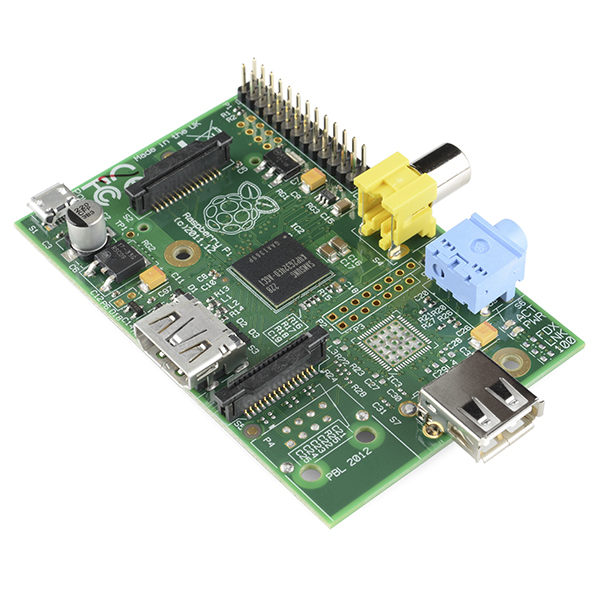
\includegraphics[scale = 1.5]{fig/Raspberry-Pi-1-modelo-A.jpg}
\caption{Raspberry Pi 1 modelo A}
\label{fig:raspberry-pi-1-modelo-a}
\end{figure}

\subsubsection{Raspberry Pi 1 modelo B}

\noindent También en 2012, la Raspberry Pi 1 modelo B apareció en el mercado trayendo el doble de memoria RAM que su predecesora, hasta los 512MB. Adicionalmente, también se le añadió un puerto USB más, y un conector RJ-45. Más tarde apareció el modelo B+, que incluía 4 puertos USB y usaba una tarjeta MicroSD, en lugar de la SD.

\subsubsection{Raspberry Pi 2 modelo B}

\noindent No fue hasta 2014 cuando hizo su aparición el siguiente modelo, la Raspberry Pi 2 modelo B, que cambió por primera vez el procesador de sus predecesoras, incorporando uno de 4 núcleos y aumentando su frecuencia hasta los 900MHz. La memoria RAM ascendió al doble de capacidad, llegando hasta 1GB. Además de todo eso, esta Raspberry Pi incluyó 40 pines GPIO y eliminó la conexión RCA. En la figura~\ref{fig:raspberry-pi-2-modelo-B} se muestra este modelo de Raspberry Pi.

\begin{figure}[tbp]
\centering
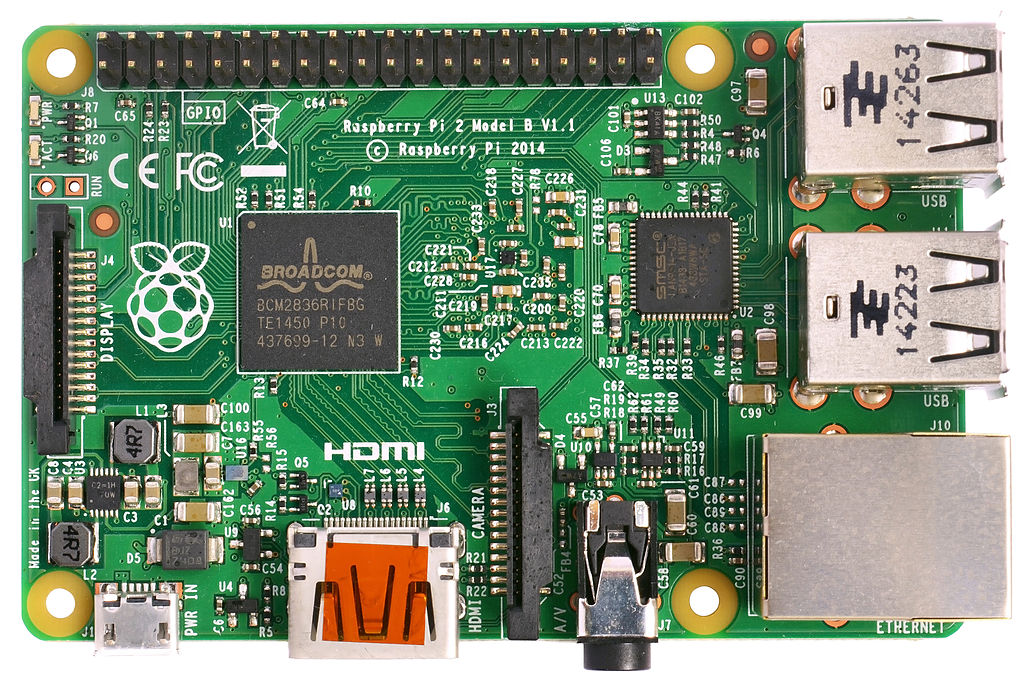
\includegraphics[scale = 1]{fig/Raspberry-Pi-2-modelo-B.jpg}
\caption{Raspberry Pi 2 modelo B}
\label{fig:raspberry-pi-2-modelo-B}
\end{figure}

\subsubsection{Raspberry Pi 3 modelo B}

\noindent Con nacimiento en 2016, la Raspberry Pi 3 modelo B llegó con un procesador nuevo y mejorado, que pasó de los 900MHz a 1.2GHz. Sin embargo, la principal novedad que traía este modelo de Raspberry Pi era la inclusión por primera vez de conexiones Wi-Fi y Bluetooth que no prescindían de adaptadores adicionales.

\subsubsection{Raspberry Pi 3 modelo B+}

\noindent A pesar de anunciarse como una actualización del modelo anterior, la Raspberry Pi 3 modelo B+ trajo diversas mejoras, entre las que se destacan las siguientes:
\begin{itemize}
\item{Mejora del procesador, que pasa de 1.2GHz a 1.4GHz}
\item{Incorporación de doble banda de 2.4GHz y 5GHz en la conectividad inalámbrica}
\item{El puerto Ethernet pasa de 100Mbits/s hasta los 300Mbits/s}
\item{Bluetooth 4.2}
\end{itemize}

\noindent Puede observarse la Raspberry Pi 3 modelo B+ en la figura~\ref{fig:raspberry-pi-3-modelo-Bplus}.

\begin{figure}[tbp]
\centering
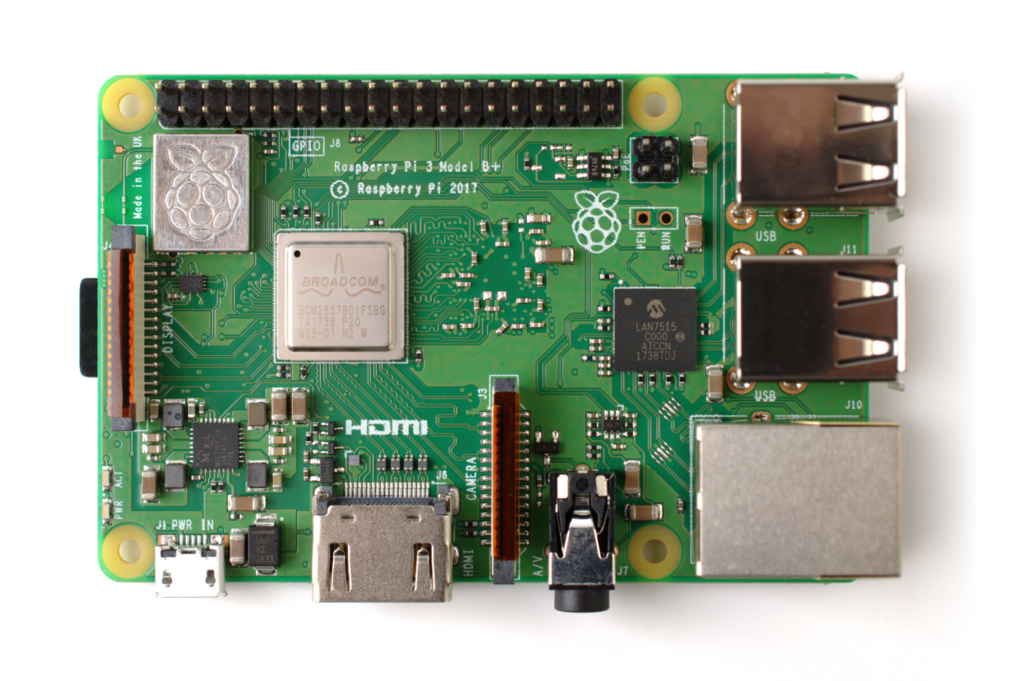
\includegraphics[scale = 0.3]{fig/Raspberry-Pi-3-modelo-B+.png}
\caption{Raspberry Pi 3 modelo B+}
\label{fig:raspberry-pi-3-modelo-Bplus}
\end{figure}

\subsubsection{Raspberry Pi 3 modelo A+}

\noindent Este modelo, que apareció en noviembre de 2018, no tenía por objeto mejorar las capacidades de sus predecesoras, si no presentar un precio más competitivo. Es por ello que, en este económico modelo contó con 512MB de RAM, un único puerto USB y eliminó la conexión RJ-45.

\subsubsection{Raspberry Pi 4 modelo B+}

\noindent Anunciada en junio de 2019, la Raspberry Pi 4 modelo B+ representa el prototipo más moderno durante la redacción de este trabajo de fin de grado. Este modelo cuenta con múltiples mejoras respecto a los modelos anteriores, entre las que pueden destacarse un procesador hasta 3 veces más eficiente que el anterior, la inclusión de una entrada USB 3.0 y el cambio de un puerto HDMI por dos puertos mini-HDMI. Este último modelo de Raspberry Pi se expone gráficamente en la figura~\ref{fig:raspberry-pi-4-modelo-B}.

\begin{figure}[tbp]
\centering
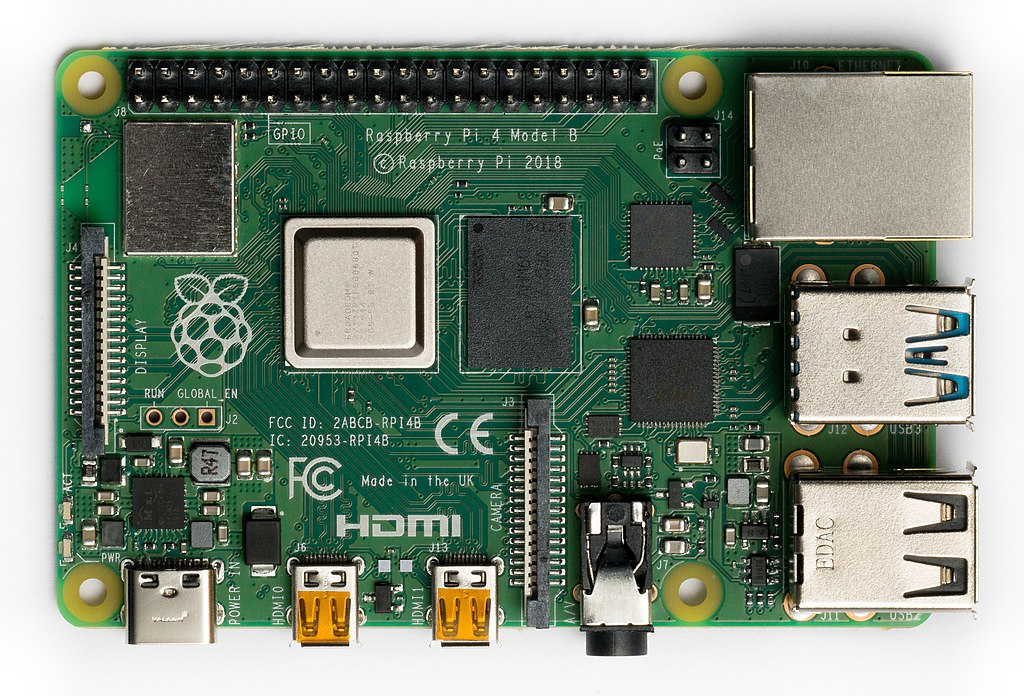
\includegraphics[scale = 0.3]{fig/Raspberry-Pi-4-modelo-B.jpg}
\caption{Raspberry Pi 4 modelo B}
\label{fig:raspberry-pi-4-modelo-B}
\end{figure}

Adicionalmente a los modelos básicos, la fundación Raspberry Pi también ha comercializado una gama de placas de menor coste y tamaño, llamadas Raspberry Pi Zero. Hasta la fecha, han aparecido tres modelos de este tipo de computadoras de bajo coste.

\subsubsection{Raspberry Pi Zero}

\noindent Hizo su aparición en 2015, y para entonces contaba ya con un procesador de 1GHz, 512MB de RAM. Debido a su diminuto tamaño, en lugar de usar los puertos HDMI y USB clásicos, hace uso de una entrada MiniHDMI y dos entradas MicroUSB. En la figura~\ref{fig:raspberry-pi-zero} se muestra esta mini computadora de bajo coste.

\begin{figure}[tbp]
\centering
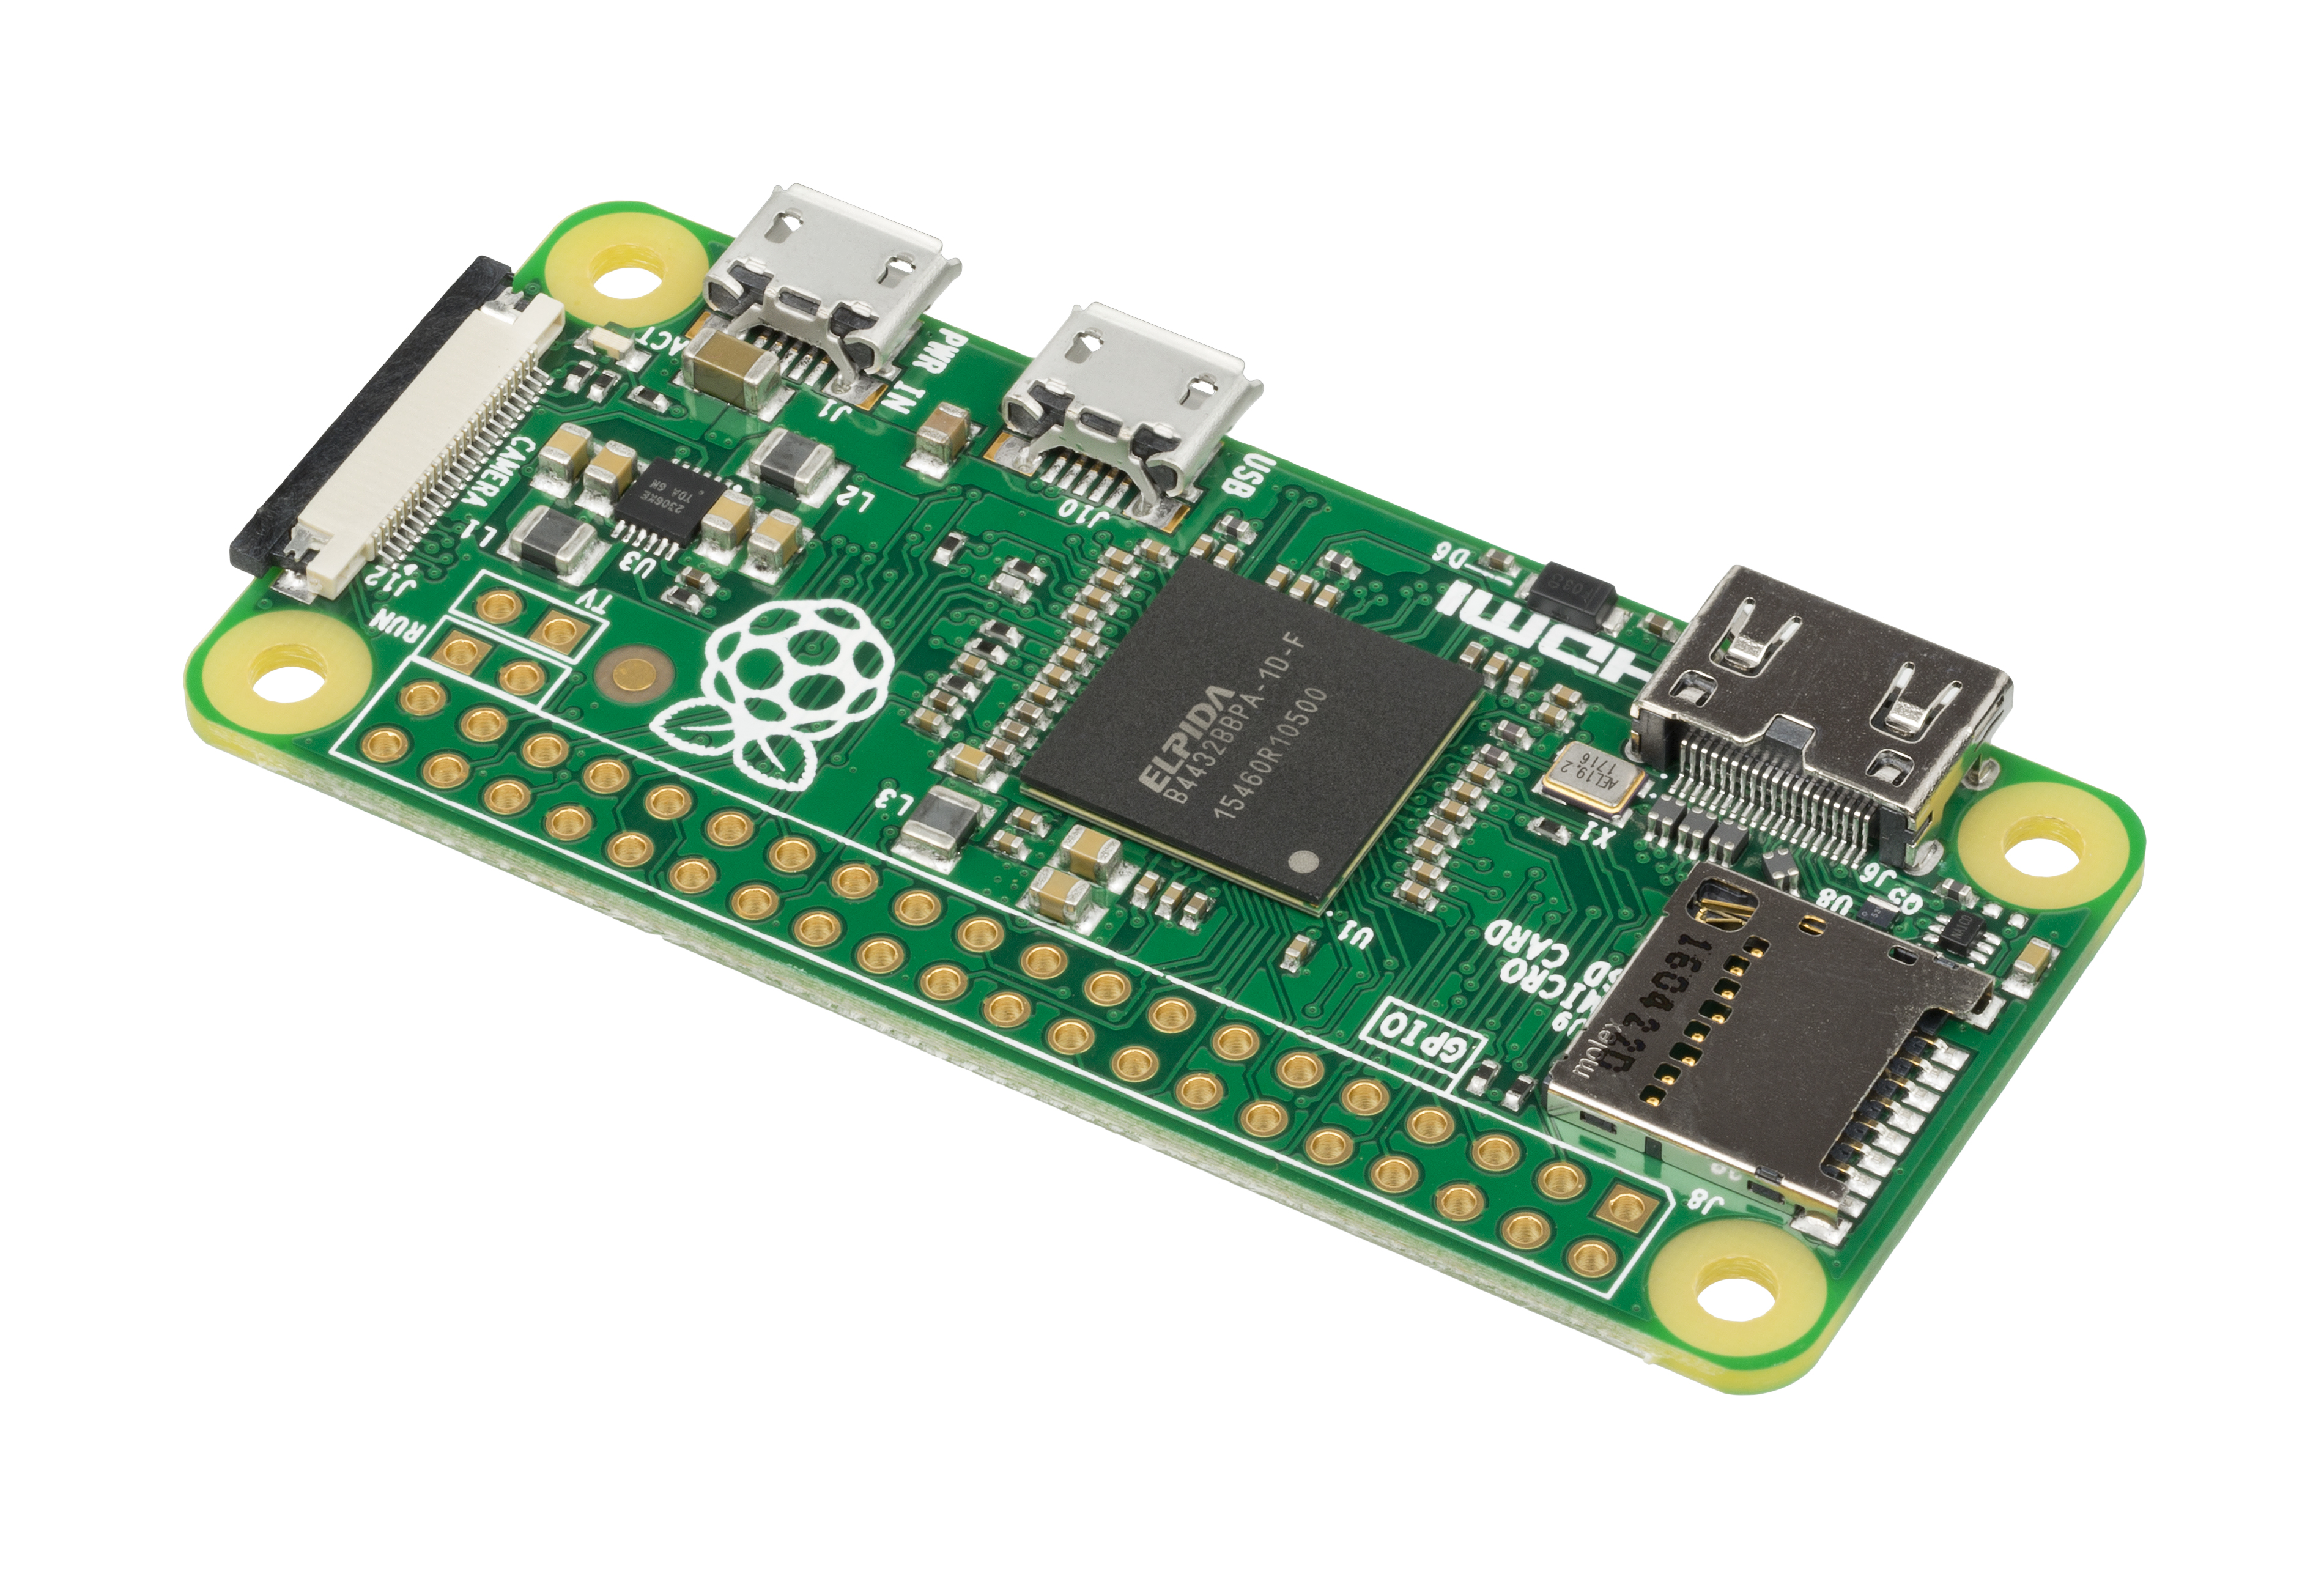
\includegraphics[scale = 0.24]{fig/Raspberry-Pi-Zero.jpg}
\caption{Raspberry Pi Zero}
\label{fig:raspberry-pi-zero}
\end{figure}

\subsubsection{Raspberry Pi Zero W}

\noindent La novedad que presenta este modelo respecto de su predecesora, es la inclusión de conexión por Bluetooth y Wi-Fi. Puede observarse este modelo de computadora en la figura~\ref{fig:raspberry-pi-zero-w}.

\begin{figure}[tbp]
\centering
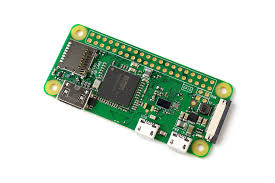
\includegraphics[scale = 1.2]{fig/Raspberry-Pi-Zero-W.jpg}
\caption{Raspberry Pi Zero W}
\label{fig:raspberry-pi-zero-w}
\end{figure}

\subsubsection{Raspberry Pi Zero WH}

\noindent Tan solo existe una diferencia entre este modelo y la Raspberry Pi  Zero W, y es la inclusión de un conector soldado a los 40 pines GPIO. Si quiere observarse la diferencia a nivel físico, no hay más que comparar esta computadora en la figura 1.7 con su predecesora en la figura~\ref{fig:raspberry-pi-zero-wh}.

\begin{figure}[tbp]
\centering
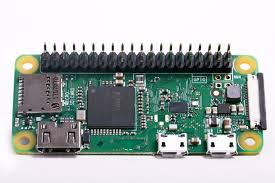
\includegraphics[scale = 0.8]{fig/Raspberry-Pi-Zero-WH.jpg}
\caption{Raspberry Pi Zero WH}
\label{fig:raspberry-pi-zero-wh}
\end{figure}

\subsection{Historia de los bots conversacionales}

\noindent En los tiempos que transcurren durante el desarrollo de este trabajo de fin de grado, los bots conversacionales parecen estar abriéndose camino a un público cada vez más amplío. Empresas como Microsoft, Google o Amazon apuestan por este tipo de tecnología, tratando de adaptarse a las necesidades de la gente con ayuda de algoritmos de inteligencia artificial.

Una buena forma de analizar la evolución de los bots, es por medio del test de Turing. En 1950, el matemático británico Alan Turing propuso un test a partir del cual se define la capacidad de un bot. La realización de dicho test consiste en ofrecer una serie de respuestas a un humano, que tendrá que decidir si estas han sido proporcionadas por otro humano o por una computadora.

Inspirado por el trabajo de Turing, el alemán Joseph Weizenbaum, desarrolló en 1966 el que sería el primer bot de la historia, al cual bautizó con el nombre de "ELIZA". Este bot consistía en un algoritmo que trataba de reconocer ciertas palabras clave, a partir de las cuales, ofrecía respuestas lógicas. Durante las pruebas conversacionales ejercidas entre humanos y ELIZA, múltiples personas creyeron estar hablando con un humano y compartieron con este bot detalles íntimos, haciendo de esta manera que ELIZA superara, a nivel teórico, el test de Turing.

De esta manera, en el 2000, apoyándose en la base establecida por sus predecesores, apareció SmarterChild, un bot capaz de procesar y entender de cierta manera el lenguaje, ofreciendo respuestas que permitían ayudar al usuario, con temas tan diversos como previsiones de meteorología o entradas de cine. SmarterChild era además compatible con plataformas de mensajería conocidas como MSN Messenger, y estableció por tanto un primer contacto entre el mundo de los bots conversacionales y el público general.

Desde entonces, la propagación de los bots, tanto de voz como escritos, se ha extendido en múltiples campos y plataformas. Desde los asistentes virtuales como Alexa y Google Home, hasta los múltiples bots de Telegram\cite{elenasantos2018} que permiten, entre otras muchas cosas, obtener imágenes de cualquier cosa con solo pedirlas o conocer la predicción meteorológica.

A finales del año 2018 ya se encontraban en funcionamiento\cite{albertoiglesiasfraga2019} más de 2.500 millones de asistentes virtuales, lo cual da muestra del estado de buena salud por el que pasa este tipo de tecnología.
